\documentclass{article}
\usepackage[a4paper, margin=2.5cm]{geometry}
\usepackage{stackengine}
\usepackage{booktabs}
\usepackage{float}
\usepackage{graphicx}
\usepackage{amsmath}
\usepackage{caption}
\def\delequal{\mathrel{\ensurestackMath{\stackon[1pt]{=}{\scriptstyle\Delta}}}}
\raggedright

\begin{document}
\today
\tableofcontents





%%%-----------------------------sections---------------------------------------%

\section{Introduction}


This paper presents an analysis of the chemical composition of 12 meteorite samples, each measured across nine key components, including metal oxides, pure metals, and carbon. Using principal component analysis (PCA), the study identifies the main sources of variation in the dataset and uncovers relationships between components, such as the opposing patterns between metal oxides and pure metals and the relatively independent role of carbon. Subcompositional analysis focuses on selected subsets of components to explore detailed interactions, while self-organizing maps (SOM) are applied to detect clustering patterns among the samples. In addition, analysis of variance (ANOVA) is used to assess which compositional balances contribute significantly to differences across grouped categories. Together, these methods provide a detailed understanding of the main chemical trends, relationships, and variation patterns present in the meteorite compositions.




\section{Data description and Visualisation}

The dataset chosen for this assignment is the meteorite compositional data. The data consists of 12 samples 
from different geographical locations see Fig. \ref{fig:locations}, each sample is composition consisting of 9 parts. The 9 parts are the metaloxides: \{FeO, Al2O3, MgO, SiO2, MnO\}, the metals \{Fw, Ni, Co\} and Carbon(C). Besides a location, each sample also had chondrite type, a summary of these can be seen in tabble \ref{tab:chondrite-types}.

\begin{table}[H]
\centering
\begin{tabular}{@{}ll@{}}
\toprule
\textbf{Code} & \textbf{Meaning} \\ \midrule
cc & \textbf{Carbonaceous chondrite}: rich in carbon, hydrated minerals, primitive, volatile-rich. \\
hc & \textbf{High-iron chondrite} (H chondrite): ordinary chondrite with high metal content. \\
lc & \textbf{Low-iron chondrite} (L chondrite): ordinary chondrite with lower metal content. \\ \bottomrule
\end{tabular}
\caption{Summary of meteorite chondrite types and their meanings.}
\label{tab:chondrite-types}
\end{table}



%Notes 
%Something abouth the fact that data is not closed to same amount
%Be clear about the fact that the data is closed for the remainder of the assignment
%Something about waht makes the data compositional 
% ALso just say something abouth the fact that there is generally a lot more of MgO SiO2 and FeO than any of the aprts:w




\begin{figure}[htbp]
    \centering
    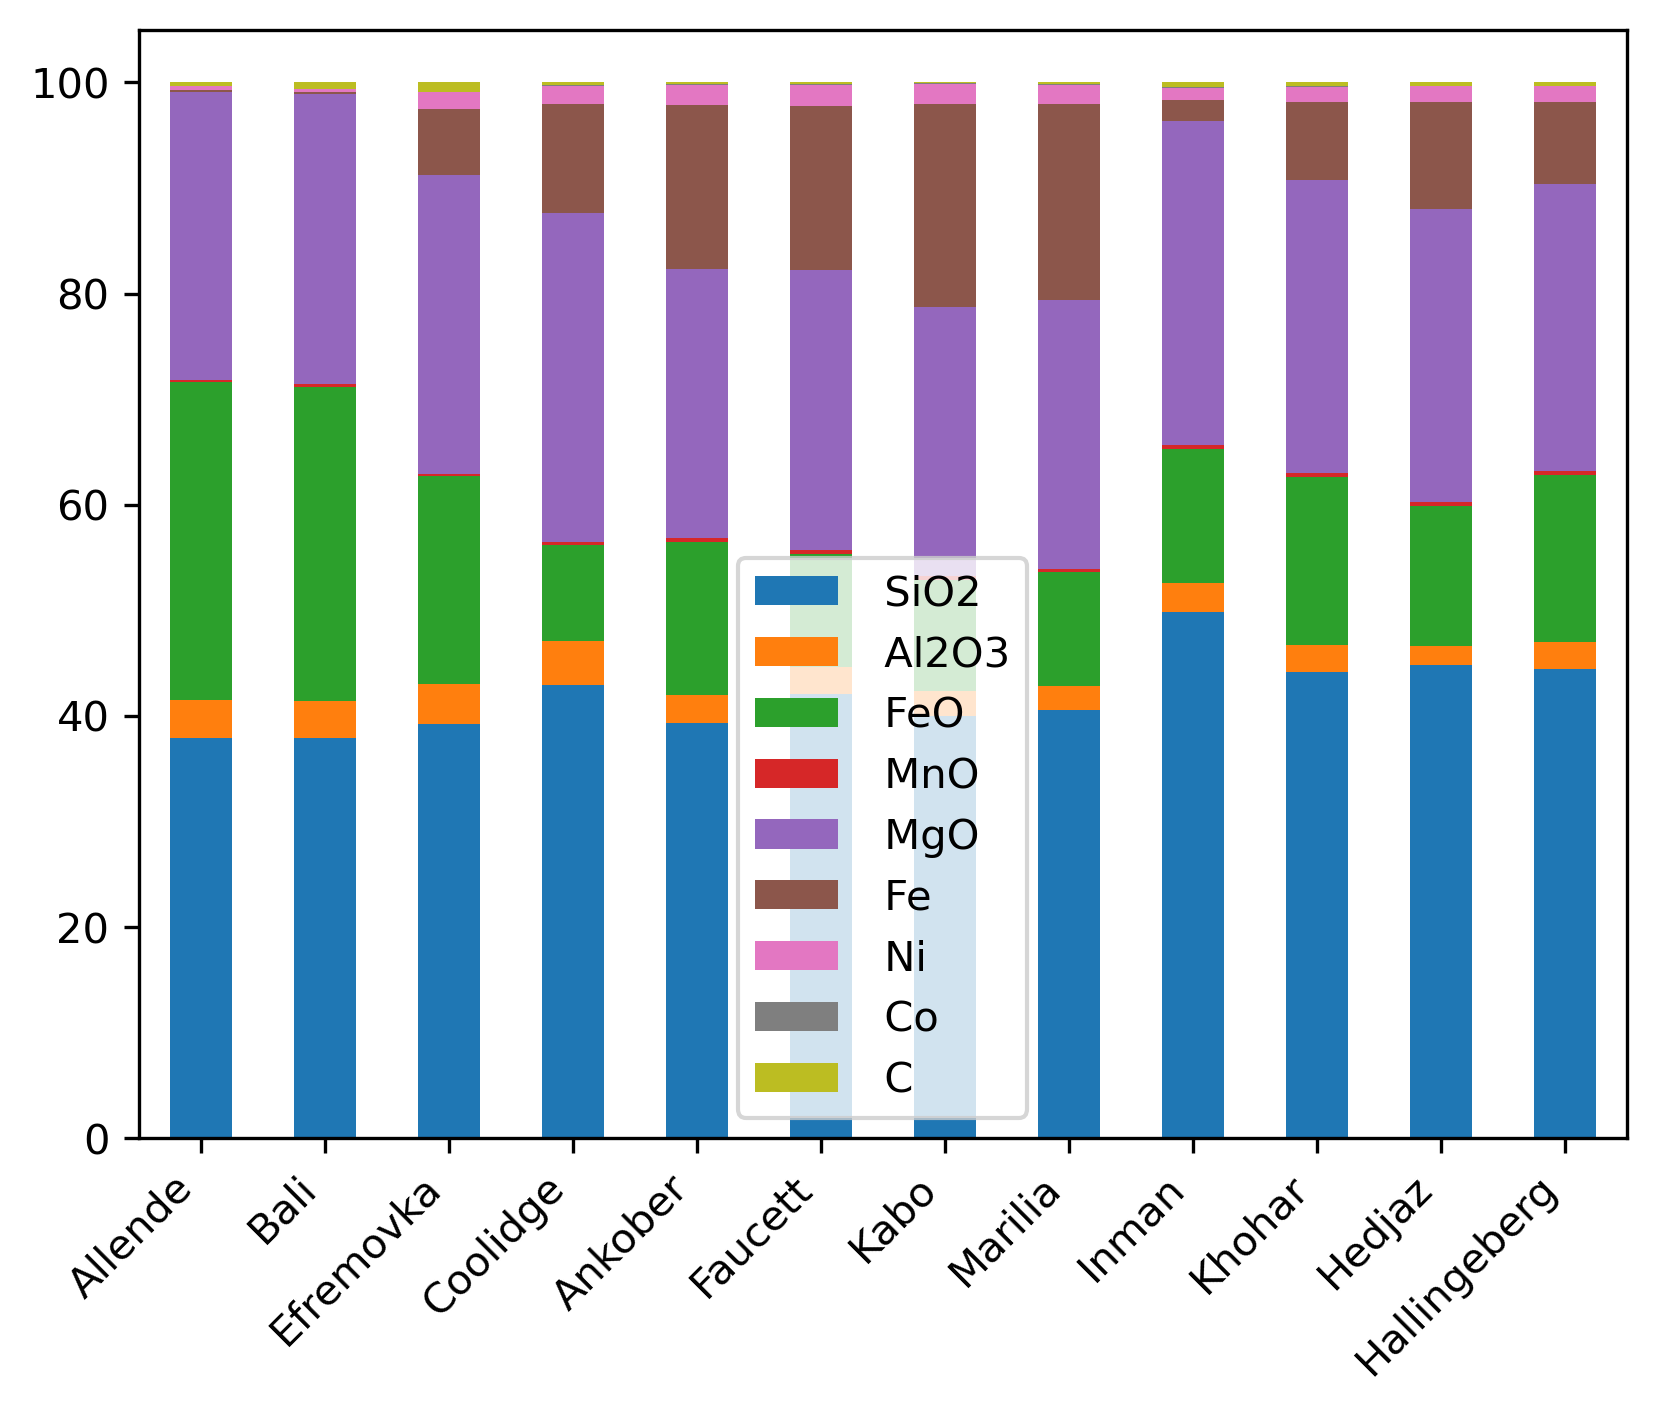
\includegraphics[width=0.8\textwidth]{figures/stacked_bar.png}
    \caption{Example plot showing the chemical composition of meteorites.}
    \label{fig:stacked}
\end{figure}






\begin{figure}[H]
    \centering
    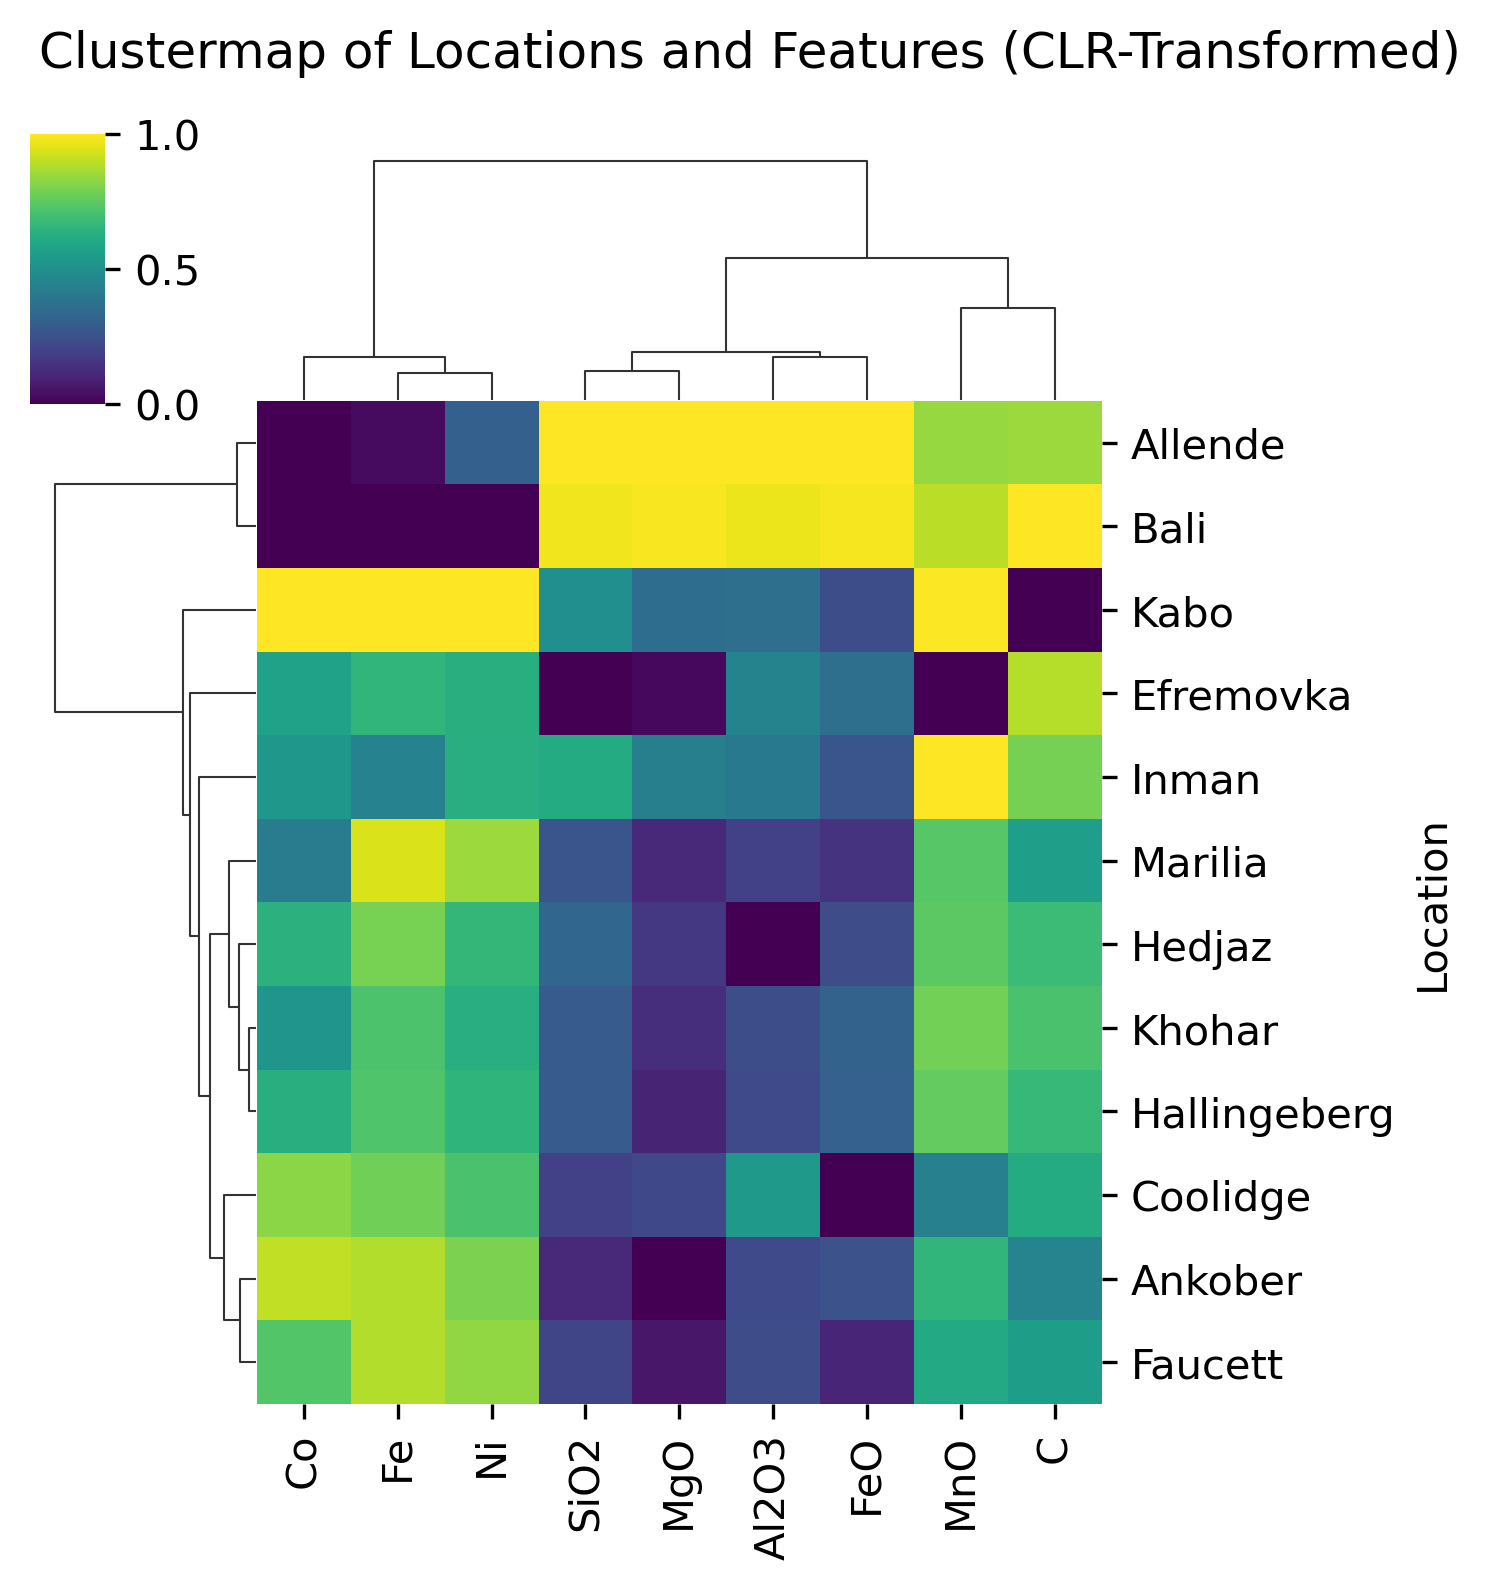
\includegraphics[width=0.4\textwidth]{figures/clustermap.png}
    \caption{Example plot showing the chemical composition of meteorites.}
    \label{fig:clustermap}
\end{figure}




\section{Exploratory data analysis}

\subsection{Principal component analysis }

To further explore patterns in the data, a Principal Component Analysis (PCA) was performed by singular value decomposition on the meteorite data.
Because PCA is very sensitive to outliers some procedures had to be performed on the data in advance of the svd. First,
the data was centered by pertubing with the geomtric mean. Next, the data was scaled by the inverse square 
root of the total variance, normalizing its overall dispersion to prevent domination by highly variable components Finally, 
the data was CLR-transformed; this step ensures that the Euclidean distance metric implied in the SVD is valid for our data.  

The PCA has been visualised using a biplot and screeplot in Fig. \ref{fig:pcabiplot}. The biplot shows the first two principal components of the data with the samples
represented as points/samples and the variables/parts as arrows. The length of the arrow indicates the importance of the variable in the PCA, and the angle between the arrows indicates how correlated they are.
The screeplot shows the proportion of variance explained by each principal component, which is useful for determining how many components to retain in the analysis. 

In this case, the scree plot shows that with only two components, we can explain 96\% of the variance in the dataset, indicating that this decomposition is highly useful for further analysis.

At first glance of the biplot we see that all the loadings of the metal oxides tend point in the same direction, this means that they are all positively correlated, while the pure metals \{Ni, Co, Fe\} is opositely correlated as the loadings of these metals points in the oposite direction of loadings of the metal oxides. This means that when we see a lot of metaloxides in a meteorite we will not see a lot of the pure metals and vice verse. The loading of Carbon on the other hand is somewhat 
perpedicular to the rest of the loadings, which suggests that there is neither a strong nor negative correlation between the 
C and the rest of the metals. 



\begin{figure}[htbp]
    \centering
    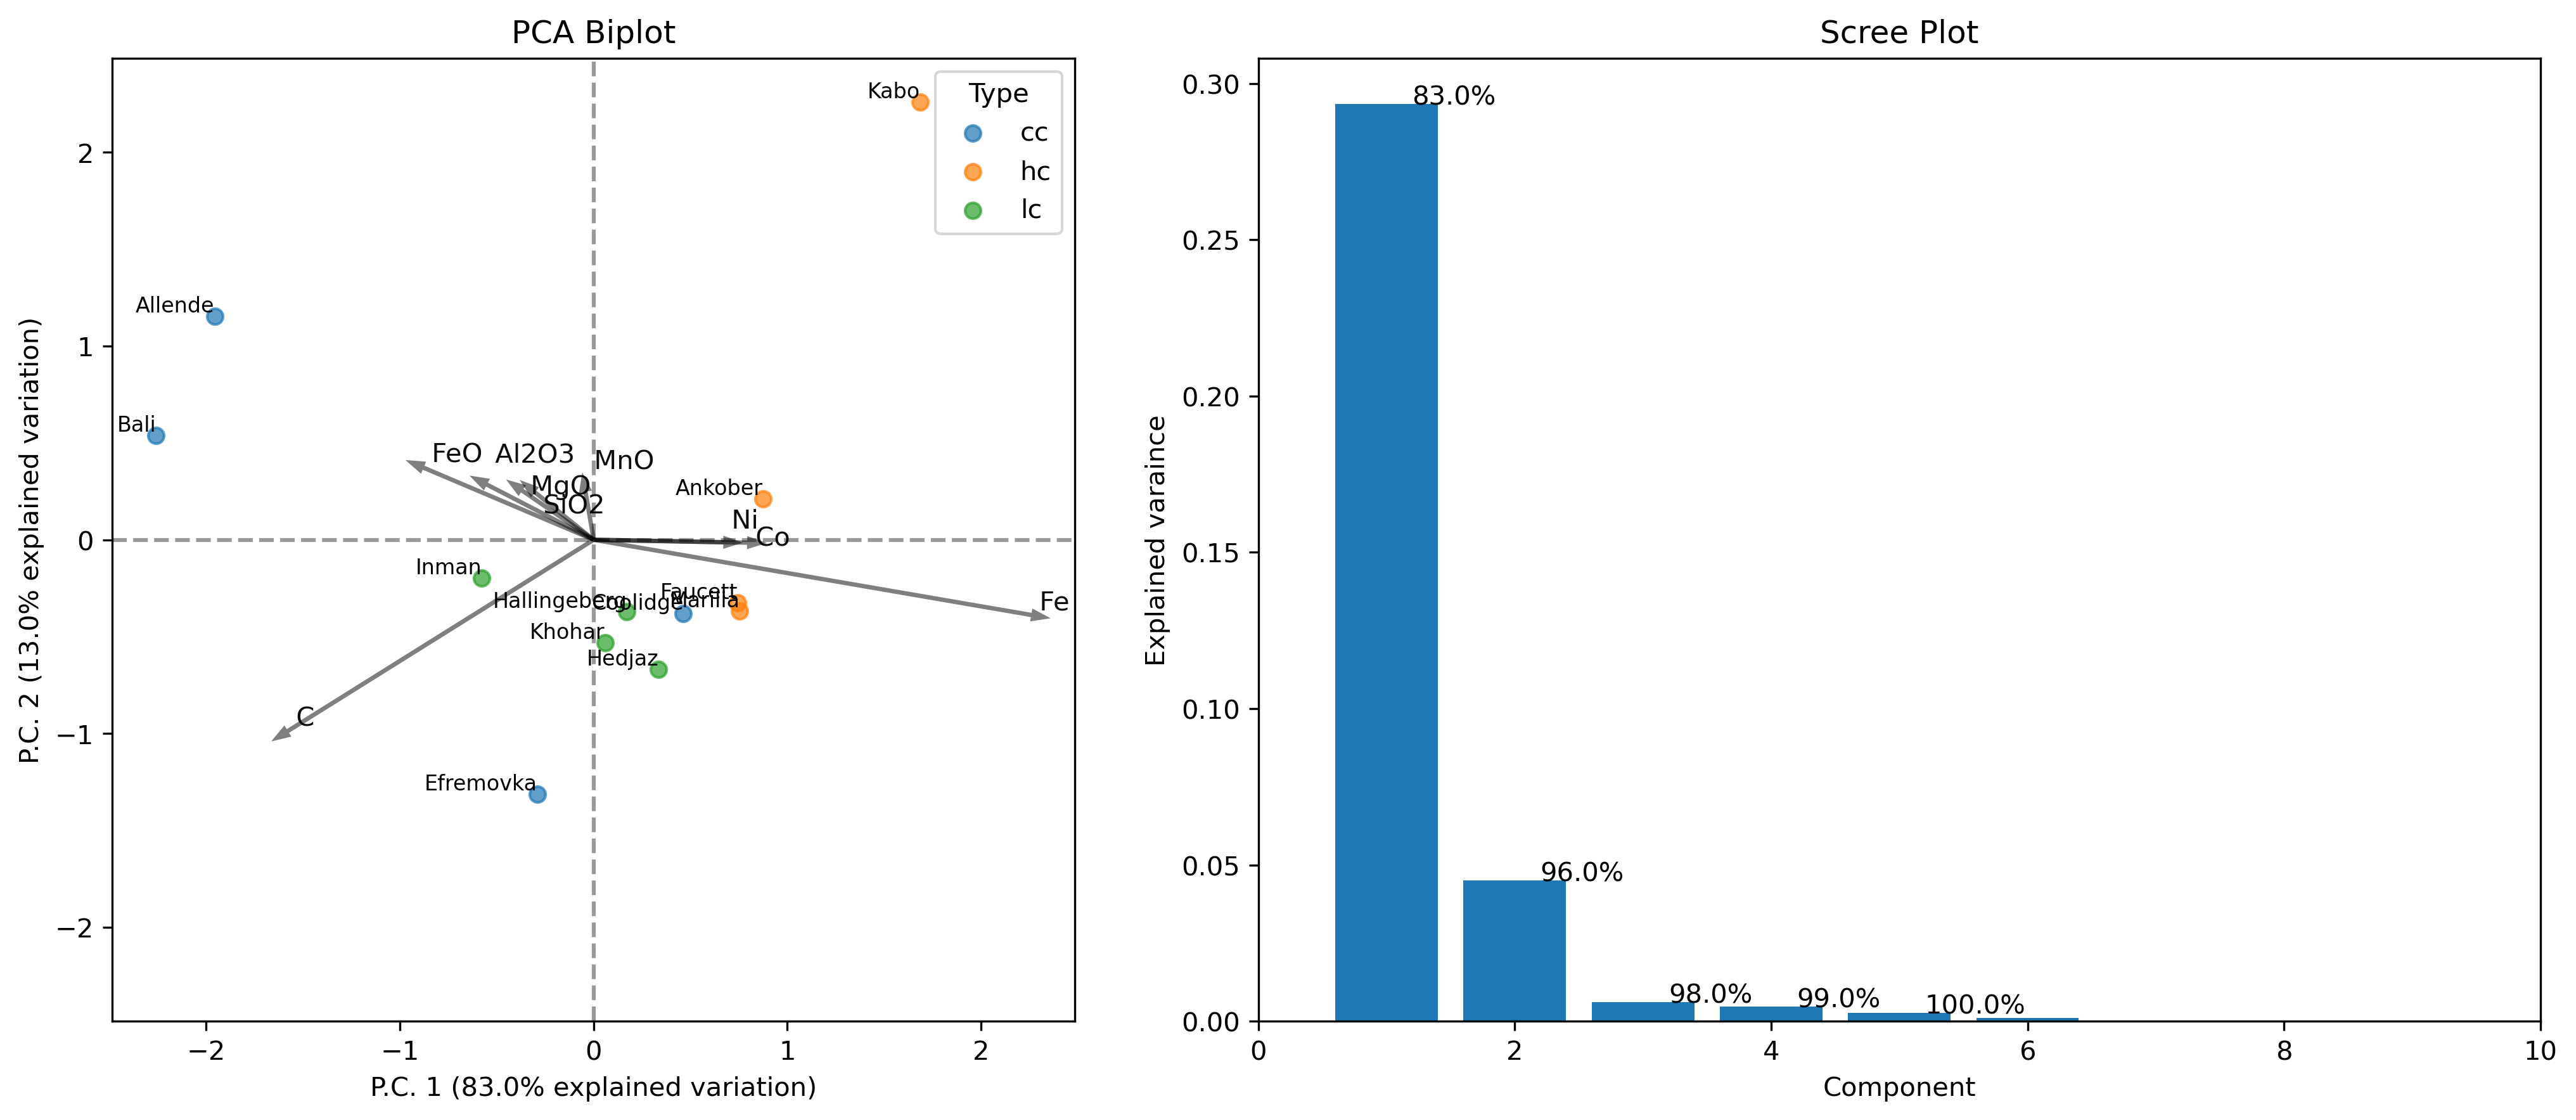
\includegraphics[width=0.8\textwidth]{figures/pca_biplot.png}
    \caption{Example plot showing the chemical composition of meteorites.}
    \label{fig:myplot}
\end{figure}
 %

\subsection{Subcompositional analysis }

From the Fig. \ref{fig:pcabiplot}, we can identify a few subcompostions where two parts loadings vertices 
are allined, the most profound of these being the Carbon loading bein perpandicular to the loadings of MgO and $SiO_2$. This subcomposition can be analysised in a ternary diagram as seen on Fig \ref{fig:ternary}. In this plot, we have first taken out the subcomposition MgO, $SiO_2$, C, applied closure to 100, center the data by pertunbation with the geometrical mean, and then finally we do a svd on this to get the eigenvalues and principal components. Additionally the explained variance of the two components was calculated by $\lambda_{i}^{2} / \sum^{i} \lambda_{i}^{2}$. PC1 describes the variation overwhelmingly well with 94.9\% of the variation in the dataset. On the ternary plot the points represents the samples from these three parts, and the line is plotted by $y = (\alpha \otimes eigenvector_{\mathrm{PC1}}) \oplus g_m$. We see high variance explained by the first PC1 in the dact that the samples are distributed very close to the line, and with a very short distance to the line indicating the very small 5.1\% captures by the PC2. 

\begin{table}[h!]
\centering
\begin{tabular}{lrrrrr}
\hline
      & MgO      & SiO$_2$   & C         & $\lambda$   & Explained Var \\
\hline
PC1   & 1.164    & 1.251     & -2.415    & 2.959       & 94.9\% \\
PC2   & 0.113    & -0.110    & -0.003    & 0.157       & 5.1\% \\
\hline
\end{tabular}
\caption{PCA Loadings and Explained Variance for MgO, SiO$_2$, and C}
\label{tab:pca_loadings}
\end{table}

\paragraph{Balance for PC2}  
The second principal component (PC2) represents the log-ratio balance between MgO and the combined contributions of SiO$_2$ and C:
\[
\mathrm{PC2} = \log\left( \frac{\mathrm{MgO}^{0.113}}{\mathrm{SiO_2}^{0.110} \, C^{0.003}} \right)
\]
This balance remains nearly constant across the dataset, reflecting that variations in MgO are proportionally matched by variations in SiO$_2$ and C, leaving only approximately 5\% of the total variance to be explained by PC2. 



\begin{figure}[H]
    \centering
    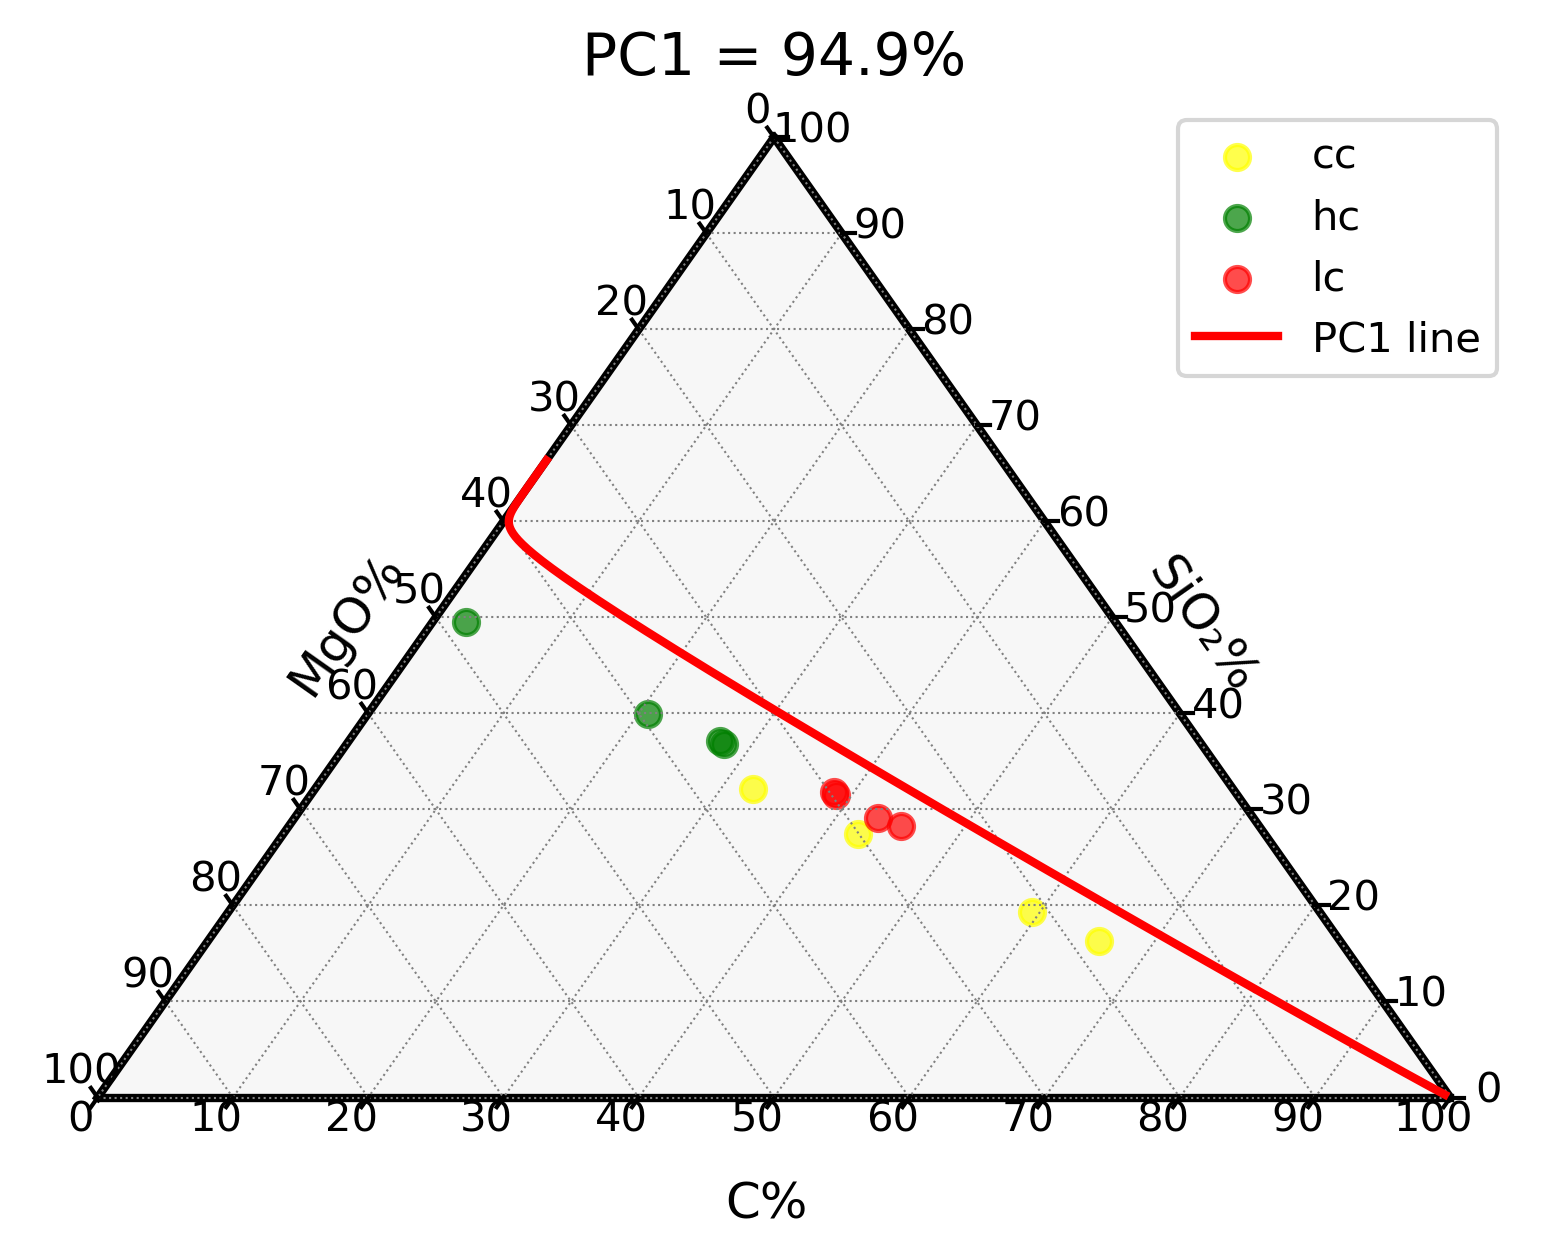
\includegraphics[width=0.8\textwidth]{figures/ternary_plot.png}
    \caption{Example plot showing the chemical composition of meteorites.}
    \label{fig:ternary}
\end{figure}


\subsection{Clusering using self organising maps}


\begin{figure}[H]
    \centering
    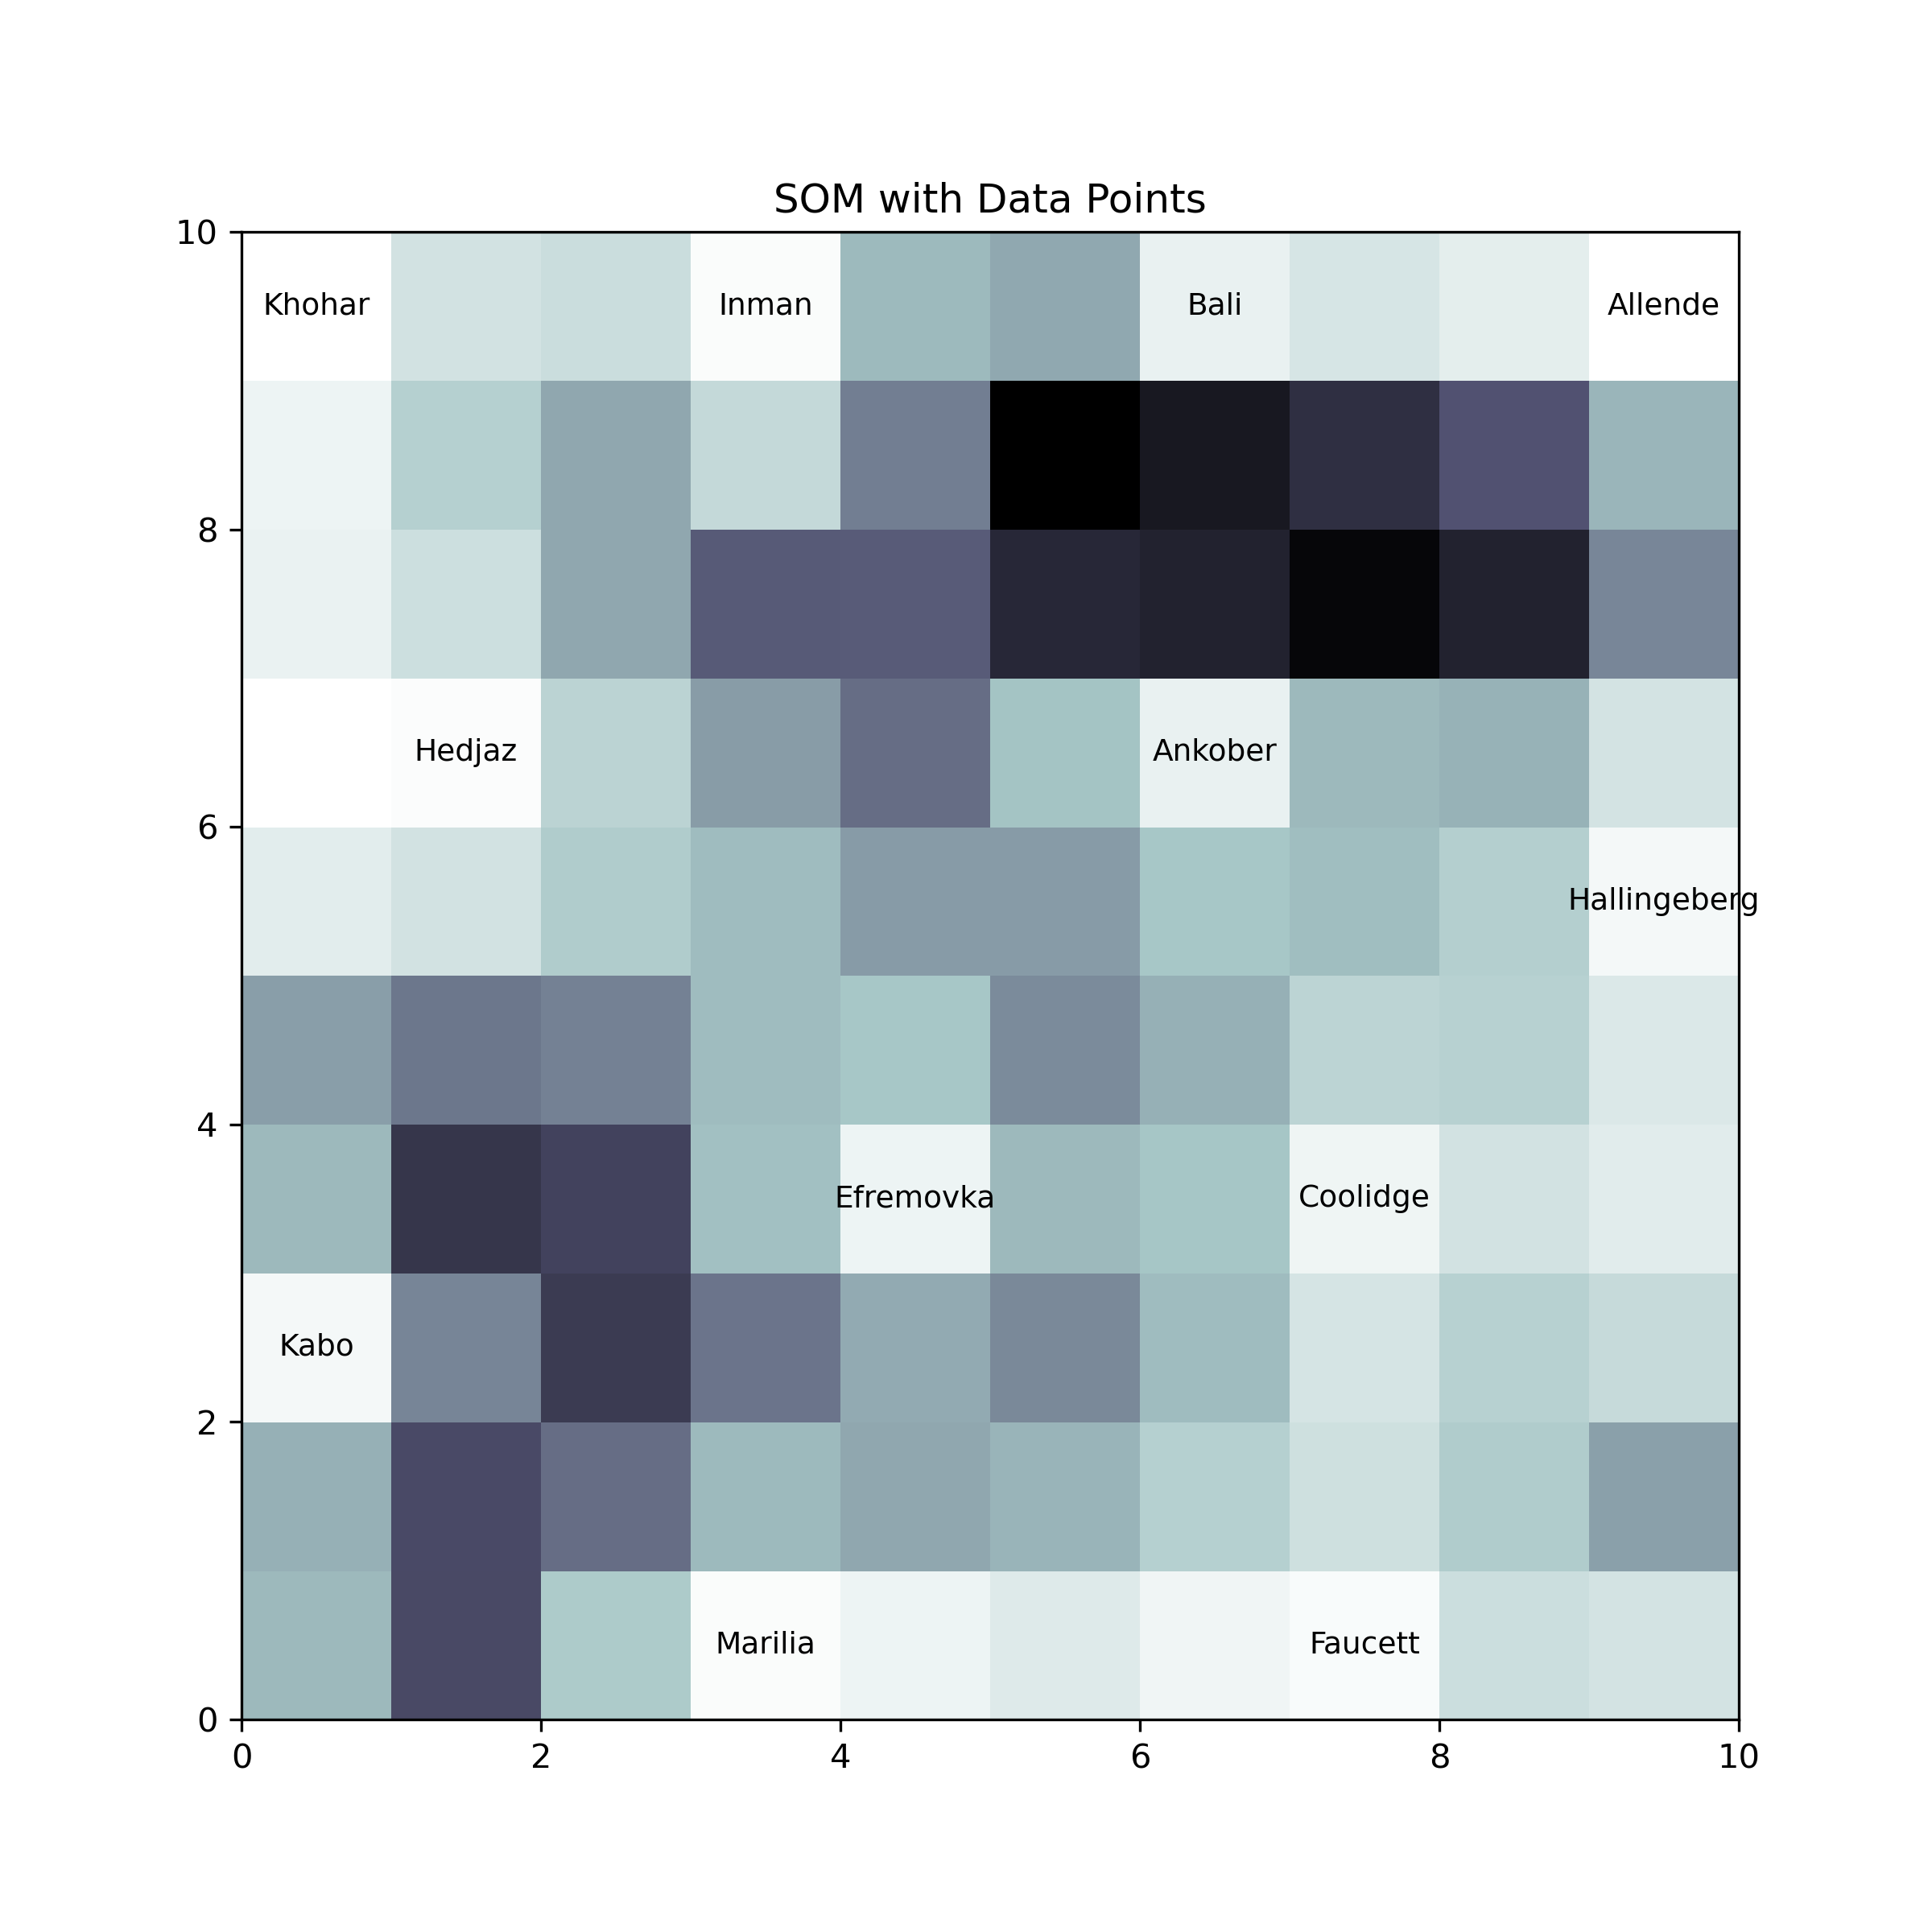
\includegraphics[width=0.5\textwidth]{figures/som_with_data_points.png}
    \caption{Example plot showing the chemical composition of meteorites.}
    \label{fig:SOM}
\end{figure}


\input{}


\begin{figure}[H]
    \centering
    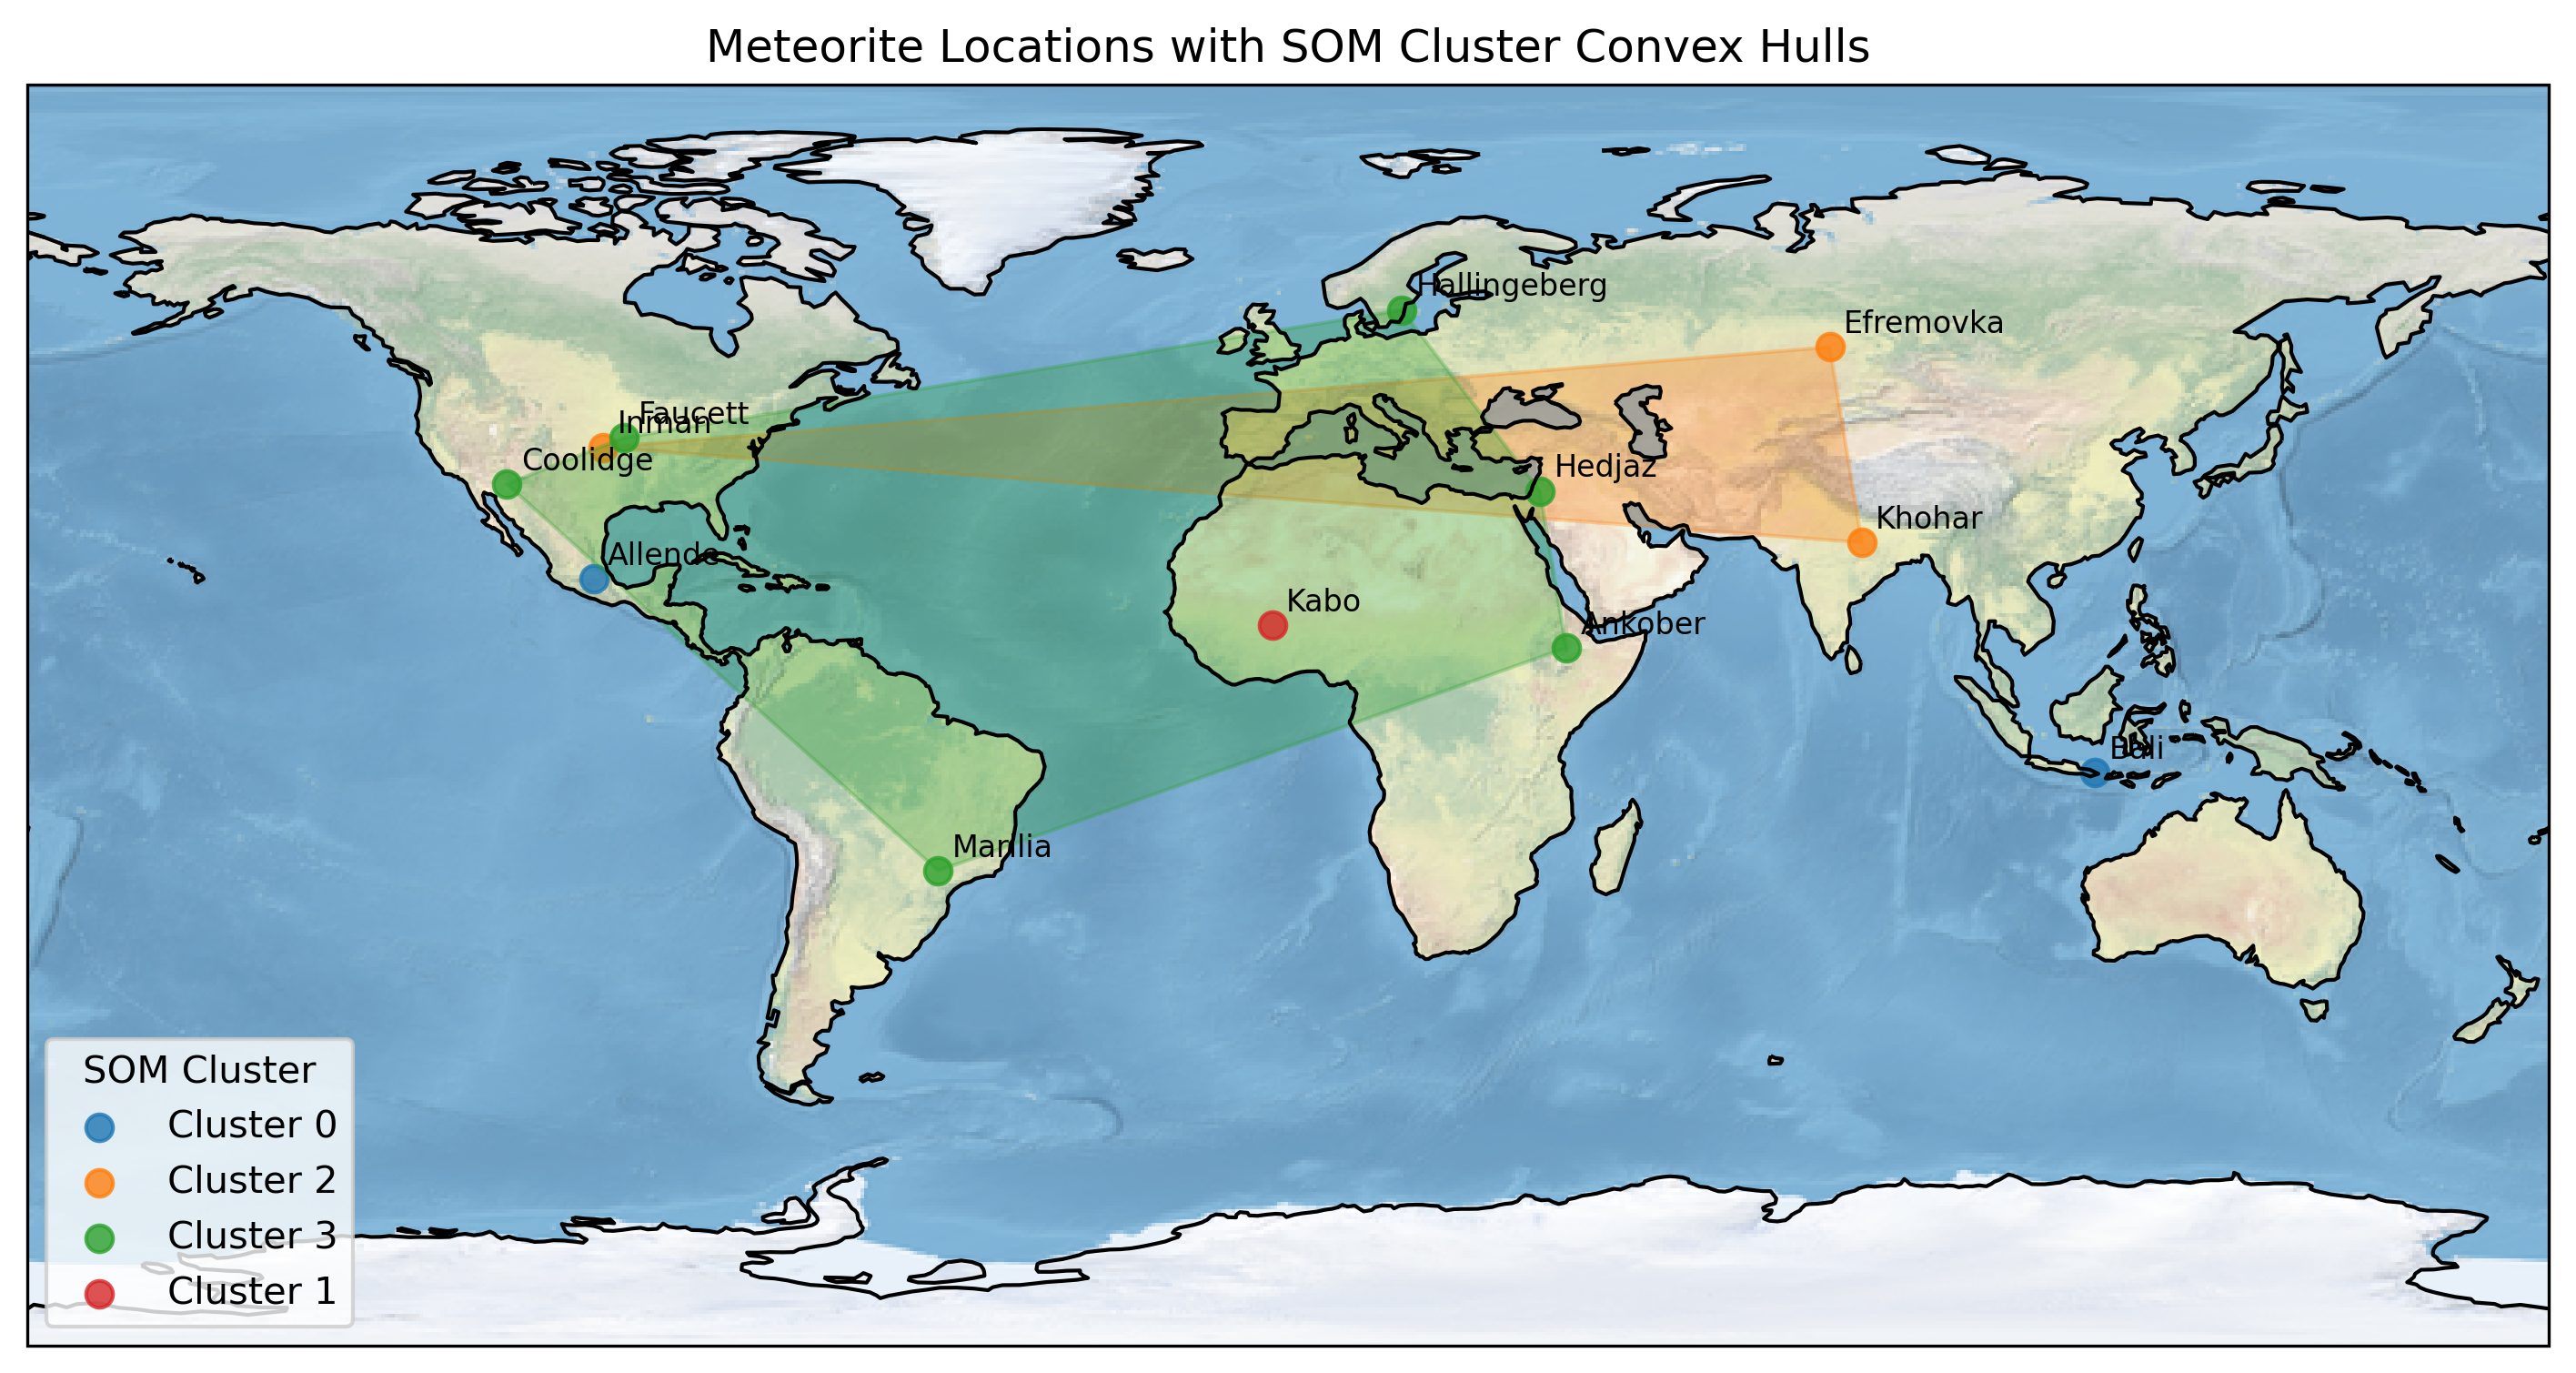
\includegraphics[width=1.0\textwidth]{figures/locations_clusters_convexhull.png}
    \caption{Example plot showing the chemical composition of meteorites.}
    \label{fig:locations_som_convexhull}
\end{figure}







\subsection{ANOVA of the chondrite types with amalgated parts}


We now want to acess which parts that contribute significantly to the difference between the chondrites types. As is stated in Table~\ref{tab:chondrite-types}, the chondrites are charerized by content of overall groups such as metals, carbons etc, consequently the parts that will be analysed for signicant impact will be the an amalgated version of the orinal parts. 

specifically the parts will be amalgated into three parts: Oxides, Metals and Carbon. To produce this supercomposition, the unclosed original 9 parts was amalgated and then closed to 100. 


To avoid having to solve the linear model: 

$$
\hat{x} = \beta_1 \oplus \left[ I(z = 2) \cdot \beta_2 \right] \oplus \left[ I(z = 3) \cdot \beta_3 \right]
$$

\noindent where:
\begin{itemize}
    \item \( \beta_1 \): baseline composition (e.g., for group 1, cc)
    \item \( \beta_2 \): perturbation for group 2 (hc)
    \item \( \beta_3 \): perturbation for group 3 (lc)
    \item \( I(z = k) \): indicator function (1 if \( z = k \), 0 otherwise)
\end{itemize}

In compositional space, the composition was first isomtric logration tranformed(ILR) using the following binary partition table:

\begin{table}[h!]
\centering
\begin{tabular}{lccc}
\textbf{Balance} & Oxides & Metals & Carbon \\
\midrule
$v_1$  & 1  & 1  & -1 \\
$v_2$  & 1  & -1 & 0  \\
\end{tabular}
\end{table}

and the betas for each part was determined using ordinary least squares. These ILR coordinates was then tranformed back to CLR for interpretation:


\begin{table}[H]
\centering
\caption{CLR Beta Coefficients for hc vs cc and lc vs cc}
\begin{tabular}{lccc}
\toprule
\textbf{Contrast} & Oxides & Metals & Carbon \\
\midrule
$CLR(\beta_{hc \, vs \, cc})$ & -0.229 & 2.078 & -1.849 \\
$CLR(\beta_{lc \, vs \, cc})$ & -0.330 & 0.908 & -0.577 \\
\bottomrule
\end{tabular}
\end{table}

A new set of binary partitions was created to explore \textbf{balances between parts showing similar effects} based on the previously obtained $CLR(\beta_2)$ (i.e., the contrast between \texttt{lc} vs \texttt{cc}). Specifically, we defined the following balances:

\begin{table}[H]
\centering
\caption{New Binary Partition Balances}
\begin{tabular}{lccc}
\toprule
\textbf{Balance} & Oxides & Metals & Carbon \\
\midrule
$v_1$ & 1 & -1 & 1 \\
$v_2$ & -1 & 0 & 1 \\
\bottomrule
\end{tabular}
\end{table}

To analyze the contribution of these balances, we performed an isometric log-ratio (ILR) transformation of the data using the new balances. We then applied ordinary least squares (OLS) regression on each ILR coordinate using the chondrite type (\texttt{cc}, \texttt{hc}, \texttt{lc}) as the covariate.

For each balance $v_i$, the OLS model is:

\[
ILR(v_i) = \beta_0 + \beta_{hc} \cdot I(\text{hc}) + \beta_{lc} \cdot I(\text{lc}) + \varepsilon
\]

where:
\begin{itemize}
    \item $\beta_0$: intercept (representing the baseline for \texttt{cc})
    \item $\beta_{hc}$: contrast (effect) of \texttt{hc} compared to \texttt{cc}
    \item $\beta_{lc}$: contrast (effect) of \texttt{lc} compared to \texttt{cc}
    \item $I(\text{hc})$ and $I(\text{lc})$: indicator functions (1 if the sample belongs to that type, 0 otherwise)
\end{itemize}

The significance of these effects was assessed using the \( t \)-values and \( p \)-values obtained from the model, as shown in Table~\ref{tab:anova_ilr_results}. As presumed from the type definitions, oxides and carbon showed a statistically significant effect in distinguishing the chondrite types, particularly between the carbonaceous (cc) and high-metal (hc) groups, as indicated by the significant \( p \)-value (0.0159) in the Oxides+Carbon balance.

Additionally, the metals balance showed a moderately significant difference (\( p = 0.0454 \)) between the groups, primarily driven by increased metal content in hc relative to cc.

These results support that both the oxide/carbon composition and the metal content are key contributors to the chemical differentiation between chondrite types, with oxides and carbon having the strongest discriminative effect.

\begin{table}[H]
\centering
\caption{ANOVA Results per ILR Balance}
\label{tab:anova_ilr_results}
\begin{tabular}{lcccc}
\toprule
\textbf{Balance} & \textbf{Intercept (cc)} & \textbf{Beta hc vs cc} & \textbf{Beta lc vs cc} & \textbf{$t$-value / $p$-value} \\
\midrule
Oxides+Carbon & 0.8793 & -2.5447 & -1.1119 & 2.6074 / 0.0159 \\
Metals & 3.7722 & 1.1458  & 0.1746  & 2.1083 / 0.0454 \\
\bottomrule
\end{tabular}
\end{table}







% section  (end)









%------------------------------------------------------------------------------------%
\newpage{}

\section{Notes}

Deadline: 12/5 kl. 14

5-10 pages incl. Figures

No collaboration


The hand-in should be emailed directly to me. The report should be a pdf or Word doc (or something similar), 5-10 pages long, including figures and tables but excluding code. I do not want to see your code, but if you must show it to me, attach the code as an appendix (which goes beyond the 5-10 pages).\newline

You are free to choose what you want to do with the dataset, as long as it falls within the scope of the course. Not all the analyses that we have discussed during lectures are relevant for all datasets, so choose something you find relevant. Maybe you need to zero-replace and maybe you want to apply closure. You most definitely want to log-ratio transform the data, but which transform you will use is up to you (depending on what you will use it for). Maybe you want to do a PCA or maybe fit a linear model or work on a sub-composition in a ternary diagram. You decide and remember that more is not necessarily better. The success criterion is that you draw some kind of (correct) conclusions on the data. Every exam dataset has been made to have some discoverable effects in them.   \newline



Dataset 2: Simple. No zeros. Look up metadata: cc, hc, lc \newline


 
\subsection{Week5 - Chapter5 - Visualisation} 
\subsection{Week6 - Chapter4 - Zero replacement} 
\subsection{Week7 - Chapter6 - Exploratory data analysis } 
\subsection{Week9 - Chapter8 - Linear analysis ANOVA} 



\section{Title}

\end{document}
